% 
% 
%			3: Preprocessing
\chapter{Preprocessing}
\label{chap:preprocessing}

First of all, some basic exploratory data analysis was performed on the data sample.


Two issues were found:

1. Missing values in \texttt{user\_id} column.
Such records were excluded.
\begin{figure}[h]
	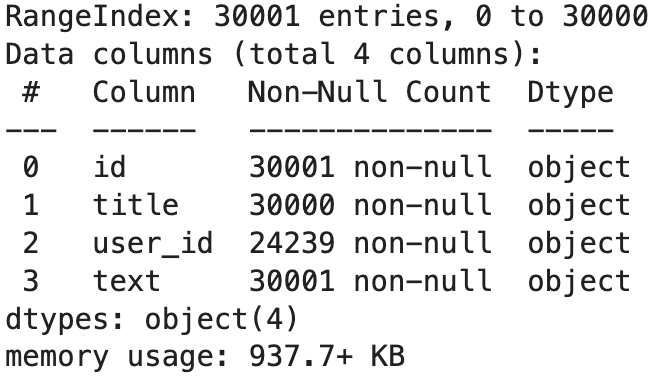
\includegraphics[width=6cm]{images/3-df_info}
\centering
\end{figure}


2. Duplicated review texts of the same book (under distinct ids) by the same user. 
Such records were excluded as they don't contain any useful information in the context of market-basket analysis of book. 

\begin{figure}[h]
	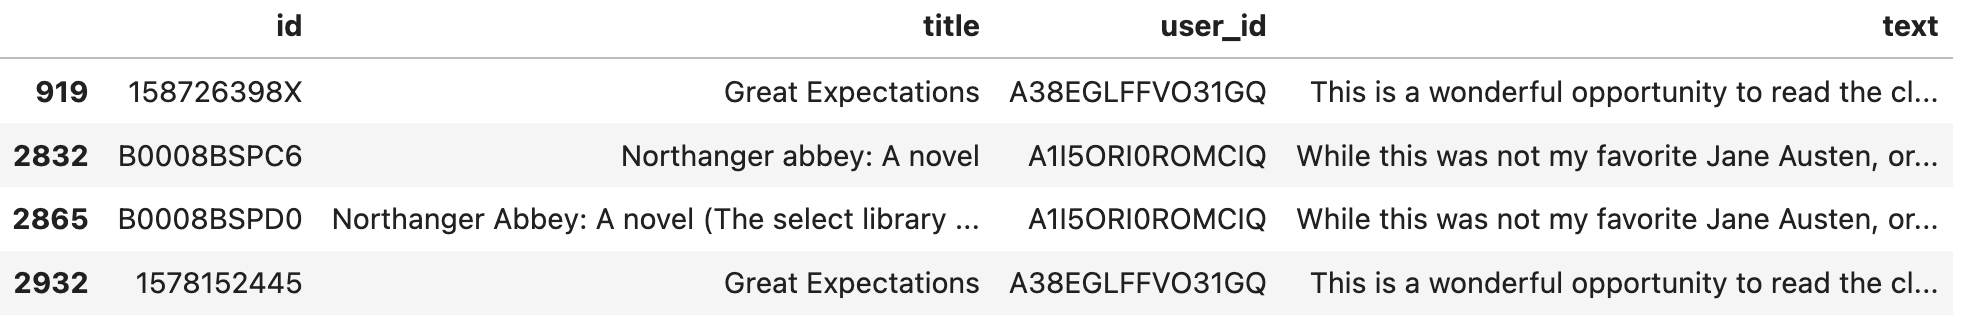
\includegraphics[width=14cm]{images/3-duplicated_reviews}
\centering
\end{figure}


The distribution of basket sizes was analysed. The vast majority of users have only one review - it means that the majority of baskets contain only one item.
Consequently, the analysis can be limited to analysing frequent pairs (doubletons).

\begin{figure}[h]
	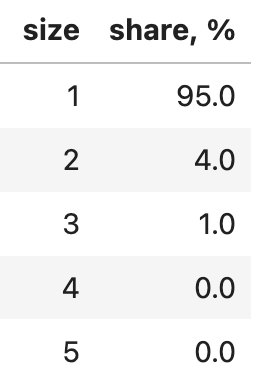
\includegraphics[width=2cm]{images/3-basket_size_histogram}
\centering
\end{figure}

\newpage



At last, string item ids were converted to integer ids to reduce RAM and CPU consumption.

\begin{figure}[h]
	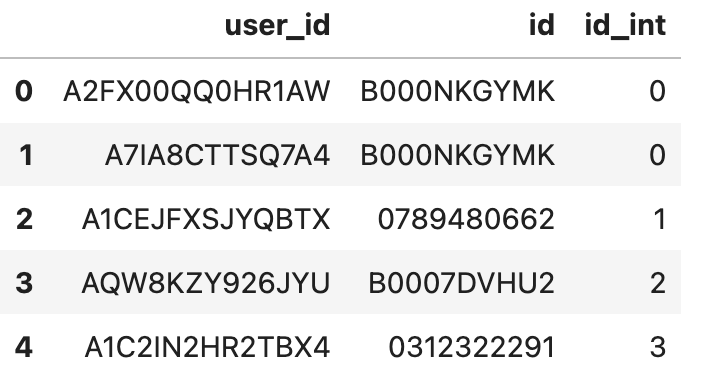
\includegraphics[width=6cm]{images/3-df_head}
\centering
\end{figure}


